Some election audits have benefited from a one-and-done approach: draw a large sample with high probability of stopping in the first round and usually avoid a second round altogether. This is appealing for two reasons. Firstly, rounds have some overhead in both time and effort. Thus the time and person-hours of an audit grows not just with the number of ballots sampled but also with the number of rounds. Secondly, smaller first round sizes are not large enough to accurately capture the distribution of votes. There is a higher probability that the true winner has fewer votes in the audit sample than some other candidate. On the other hand, a one-and-done audit may draw more ballots than are necessary; a more efficient round schedule could require less effort and time pre-certification. To evaluate the quality of various round schedules, we construct a simple workload model. Using this model we show how optimal round schedules can be chosen. We provide software that can be used by election officials to choose round schedules based on estimates of the model parameters like maximum allowed probability of a misleading audit sample.

As an example, we consider the US Presidential contest in the 2016 Virginia statewide general election. This contest had a margin of $0.053$ between the two candidates with the most votes.
Analytical approximation of the expected audit behavior (quantities like expected total number of ballots sampled or total number of rounds) is not straightforward. %challenging because the number of possible sequences of samples grows exponentially with the number of rounds. 
%A very rough approximation scheme is possible and may be useful when choosing round sizes in practice. We implement such a scheme, available at \cite{software}.
%We will use the more standard approach of simulations to give an example here.
Therefore we use the typical approach of simulations, again with risk limit $0.1$.

We simulate audits considering each candidate with a column in the results available at the Virginia Department of Elections website, including irrelevant ballots.
We consider a simple round schedule, in which each round is selected to give the same probability of stopping, $p$. That is, if the audit does not stop in the first round, we select a second round size which, given the sample drawn in the first round, will again have a probability of stopping $p$ in the second round. Note that since there are multiple candidates, we compute the minimum round size to achieve stopping probability $p$ for each pairwise contest between the winner and one of the losers, and we then select the largest such minimum round size and scale it up according to the proportion of the total ballots that are relevant to that pairwise contest. For this round schedule scheme, a one-and-done audit is achieved by choosing large $p$, say $p=.9$ or $p=.95$. We run $10^4$ trial audits for each value of $p$, assuming the reported results are correct\footnote{For this particular round schedule scheme, computing the expected number of rounds is straightforward analytically, but the expected number of ballots is still difficult, and so we use simulations.}. 

Note that simulations of audits of tied elections are not necessary, as all the audits we are considering are risk-limiting and hence we already know the performance to expect when auditing a tied election, even one not reported as such. 

Importantly, note that \Minerva does not appear in the analysis in this section. 
Questions about the efficiency of \Minerva for its necessarily fixed round schedules are addressed in section~\ref{sec:sims}, but in this section round sizes are chosen to have specified probabilities of stopping given previous samples. \Minerva is not known to be risk-limiting in this setting, and thus cannot be used for RLAs that proceed in this way.

\subsection{Person-hours}

\subsubsection{Average total ballots.} 
The simplest workload models are a function of just the total number of a ballots sampled\footnote{Sometimes total \emph{distinct} ballots sampled is used, but for the margins we use in our examples in this section, the difference between total distinct ballots and total ballots is very small\cite{arxiv_athena}. It is straightforward to modify the model we discuss here to account for total distinct ballots.}. Figure~\ref{fig:avg_bals} shows the average total number of ballots sampled as a function of $p$.
\begin{figure}[h!]
%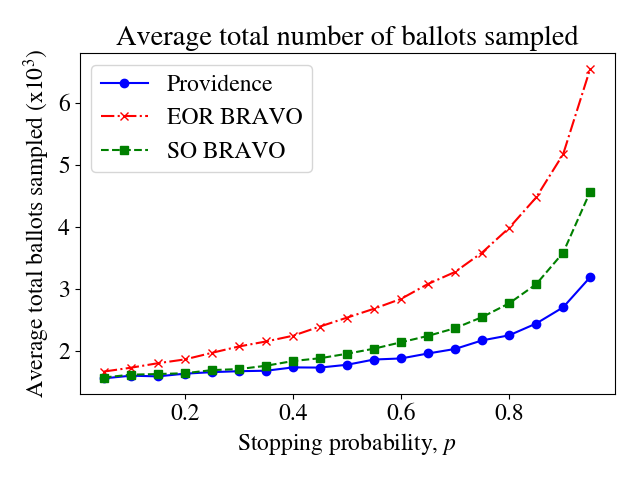
\includegraphics[width=.5\textwidth]{avg_bals.png}
%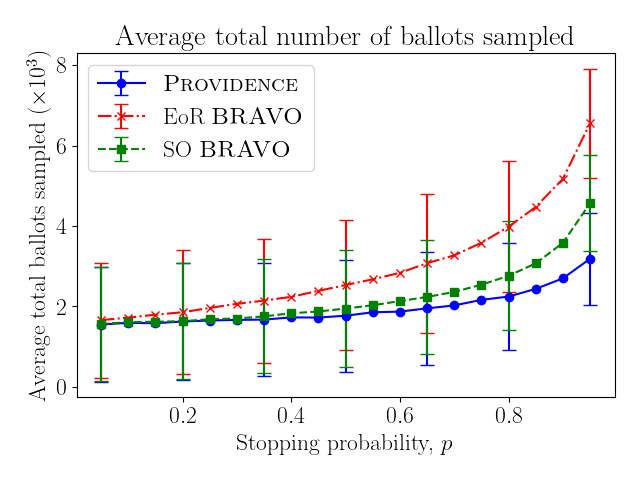
\includegraphics[width=.5\textwidth]{avg_bals_error_bars_every_three.png}
%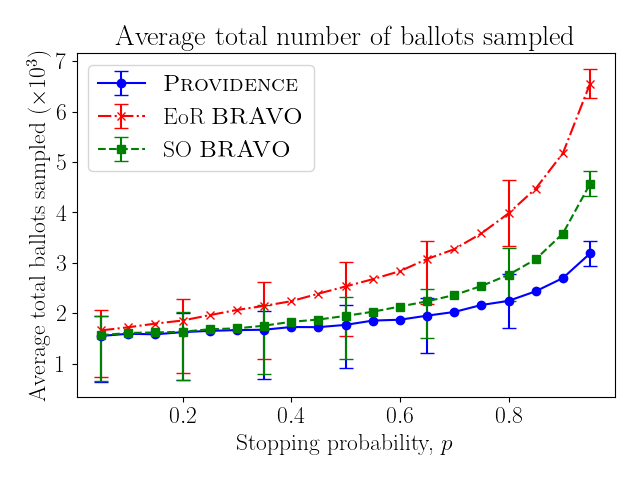
\includegraphics[width=.5\textwidth]{avg_bals_errorbars.png}
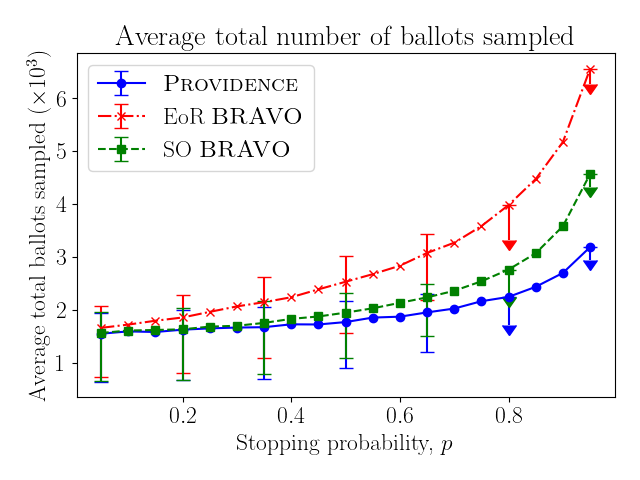
\includegraphics[width=.5\textwidth]{avg_bals_quantiles.png}
\caption{The average total number of ballots sampled, as a function of $p$, the conditional stopping probability used to select each round size, for ballot polling audits of the 2016 US Presidential election in the US State of Virginia. Error bars show the $0.25$ and $0.75$ quantiles. For sufficiently large $p$ ($p\ge 0.75$), the $0.25$ and $0.75$ quantiles are both equal to the first round size, and this is shown by the downward arrows.}
\label{fig:avg_bals}
\end{figure}

%Figure~\ref{fig:avg_bals_ratio} provides the same number as a fraction of the \Providence values.
It is straightforward to show that \Providence and both forms of \BRAVO collapse to the same test when each round corresponds to a single ballot. Figures~\ref{fig:avg_bals} 
%and \ref{fig:avg_bals_ratio} 
shows that for larger stopping probabilities $p$ (i.e. larger rounds), \Providence requires fewer ballots on average. In particular, the savings of \Providence become larger as $p$ increases; for $p=0.95$, EoR \BRAVO and SO \BRAVO require more than $2$ and $1.4$ times as many ballots as \Providence respectively. 

%\begin{figure}[h!]
%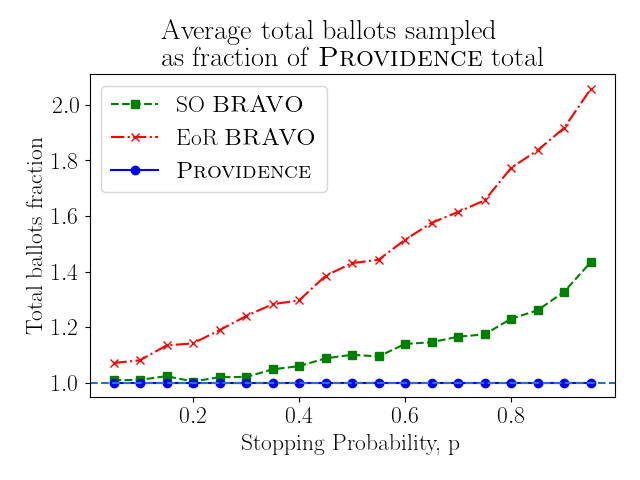
\includegraphics[width=.5\textwidth]{avg_bals_ratio.png}
%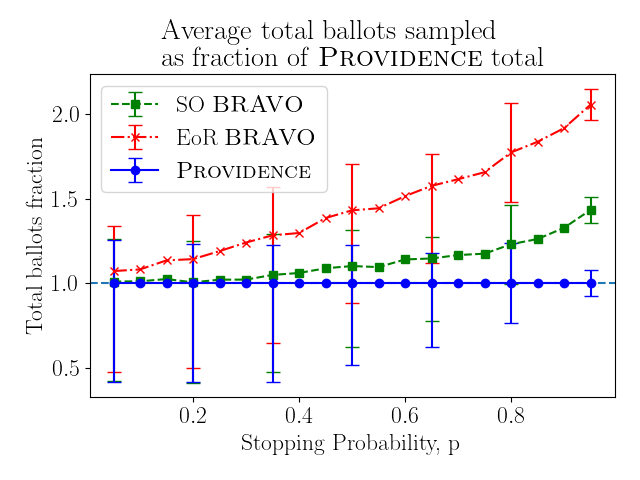
\includegraphics[width=.5\textwidth]{avg_bals_ratio_errorbars.png}
%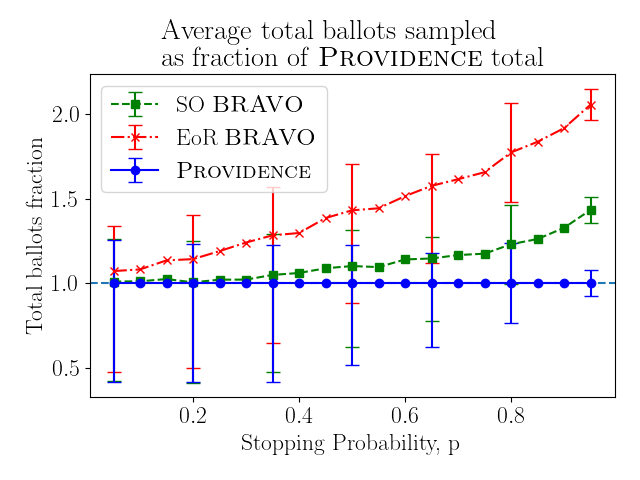
\includegraphics[width=.5\textwidth]{avg_bals_ratio_errorbars.png}
%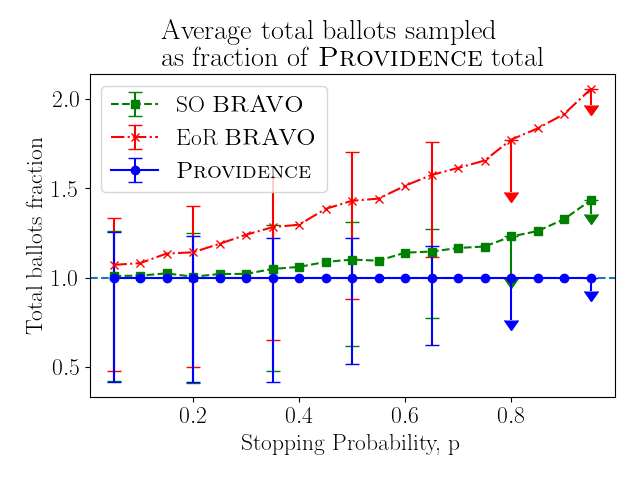
\includegraphics[width=.5\textwidth]{avg_bals_ratio_quantiles.png}
%\caption{The total number of ballots sampled on average, as a fraction of those sampled by \Providence, as a function of $p$, the conditional stopping probability used to select each round size, for ballot polling audits of the 2016 US Presidential election in the state of Virginia. The $0.25$ and $0.75$ quantiles are shown as in Figure~\ref{fig:avg_bals}.}
%\label{fig:avg_bals_ratio}
%\end{figure}


\subsubsection{Round overhead.} 
It is clear that average number of ballots alone is an inadequate workload measure. 
(Consider a state conducting its audit by selecting a single ballot at random, 
notifying just the county where the ballot is located, and then waiting to hear back for the manual interpretation of the ballot before moving on to the next one. 
This of course is inefficient and is why audits are actually performed in rounds.)

In a US state-wide RLA, the state organizes the audit by determining the random sample and communicating with the counties, but election officials at the county level physically sample and inspect the ballots after drawing them from secure storage boxes stored in county locations. 
Therefore each audit round requires some number of person-hours for set up and communication between state and county. This overhead for a round includes choosing the round size, generating the random sample, and communicating that random sample to the counties, as well as the communication of the results back to the state afterwards. 

Consequently, we now consider a model with a constant per-ballot workload $w_b$ and a constant per-round workload $w_r$.
So for an audit with expected number of ballots $E_{b}$ and expected number of rounds $E_{r}$, we estimate that the workload $W$ of the audit is
\begin{equation}
W(E_b,E_r) = E_b w_b + E_r w_r + C
\label{eq:round_workload}
\end{equation}

Note there is also some constant overhead of workload for the whole audit, namely $C$ in Equation~\ref{eq:round_workload}, which we take to be zero in our examples but could be used by election officials to represent, for example, the effort of constructing a ballot manifest.
For simplicity, (and without loss of generality), we measure in multiples of the per ballot workload; that is, we assume it is one unit, $w_b=1$. A per round workload of $w_r=x$ corresponds to a per round workload which is $x$ times the per ballot workload. We use $w_r=1000$ as a conservative example. 
That is, we set the overhead of a round equal to the workload of sampling $1000$ ballots. Based on available data\cite{RI-report}, the time retrieving and analyzing each individual ballot is on the order of $75$ seconds which means that $w_r=1000$ is equivalent to roughly $20$ person-hours of workload. This corresponds to about $15$ minutes being spent, on average, per round in each of the $133$ counties of Virginia, a clearly conservative workload estimate. We do not consider $w_r < 1$ because it is not possible for the round overhead to be smaller than the workload corresponding to a single ballot. 

As shown in Figure~\ref{fig:with_round_workload}, average workloads first reduce as stopping probability increases; this is likely due to a decrease in the number of rounds. After hitting a sweet spot, average workloads again increase with stopping probability; this time, likely because the average number of rounds does not decrease much and the cost changes because of number of ballots drawn, which increases with round size. \Providence achieves the lowest minimum average workload at roughly $p=0.7$ for our example choice of $w_r=1000$.

\begin{figure}[h!]
%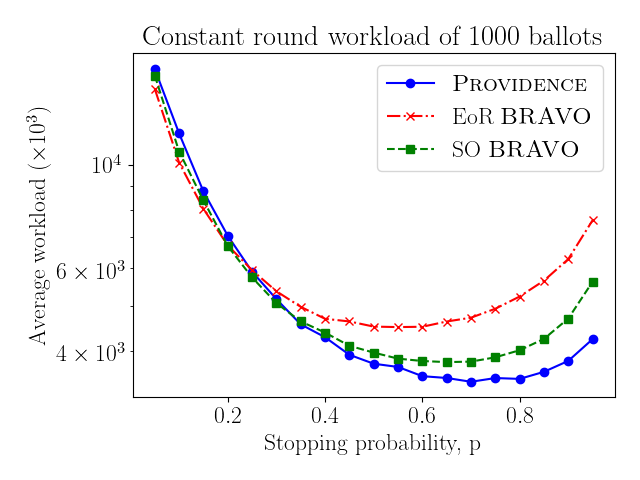
\includegraphics[width=.5\textwidth]{with_round_workload.png}
%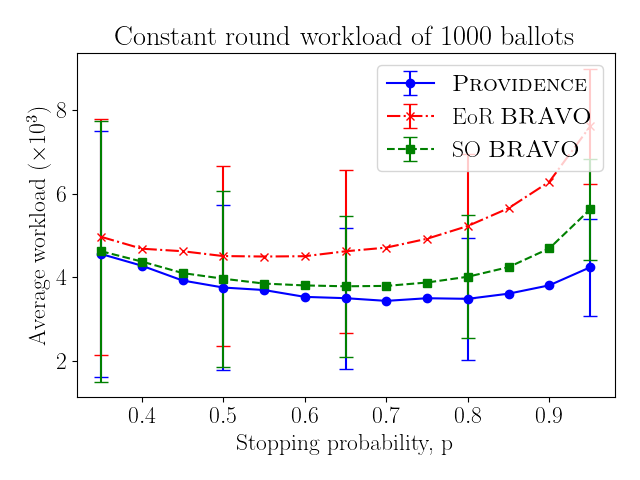
\includegraphics[width=.5\textwidth]{with_round_workload_errorbars.png}
%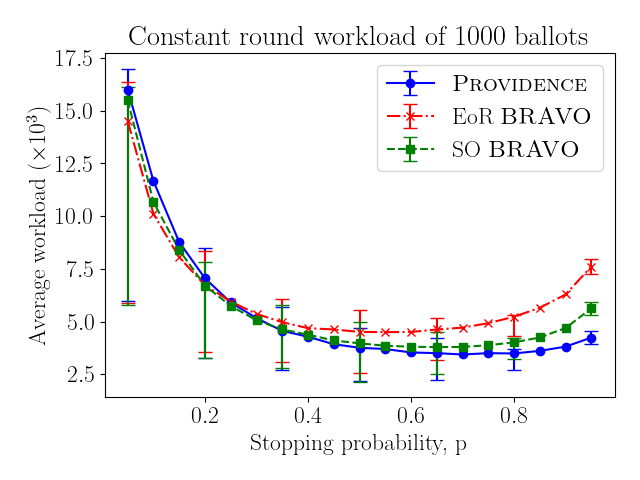
\includegraphics[width=.5\textwidth]{round_workload_errorbars.png}
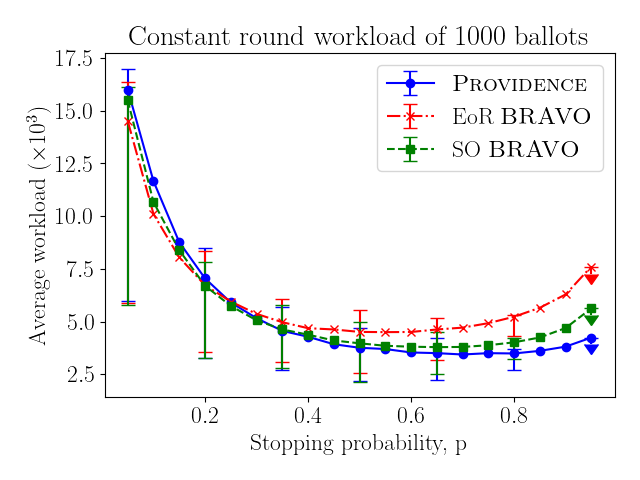
\includegraphics[width=.5\textwidth]{round_workload_quantiles.png}
\caption{For workload parameters $w_b=1$ and $w_r=1000$, this plot shows the expected workload for various values of $p$. Expected workload is found using Equation~\ref{eq:round_workload} and the average number of ballots and rounds in our simulations as the expected number of ballots and rounds. The $0.25$ and $0.75$ quantiles are shown as in Figure~\ref{fig:avg_bals}.}
\label{fig:with_round_workload}
\end{figure}

Importantly, this gives us a way to estimate the minimum expected workload, as well as which round schedule value $p$ achieves it, for arbitrary round workload. For each round workload $w_r$, we produce a dataset analagous to that of Figure~\ref{fig:with_round_workload} and then find the minimum average workload achieved for each of the audits and its corresponding stopping probability $p$. 

Figure~\ref{fig:optimal_workloads} shows the optimal achievable workload for a wide range of per round workloads. For very low round workloads, the workload function approaches just the total number of ballots, and so workload is minimized by minimizing the number of ballots drawn, which corresponds to small round sizes, and we would expect all three audits to behave similarly, as ballot-by-ballot audits, with the smallest workload. On the other hand, for extremely large values of round workload, the average number of ballots has little impact on the workload function, and so the three audits again have similar values, all corresponding to large round sizes in order to minimize the number of rounds.  We know that there is variation in the number of ballots used by each type of audit for large round sizes (a factor of two for $p=0.9$), but these values would be small in comparison to $w_r$. We observe this behaviour in Figure~\ref{fig:optimal_workloads} for extremely small and large workload values. For more reasonable values of the round workload $w_r$, SO \BRAVO and EoR \BRAVO achieve minimum workload roughly $1.1$ and $1.3$ times greater than that of \Providence.
\begin{figure}[h!]
%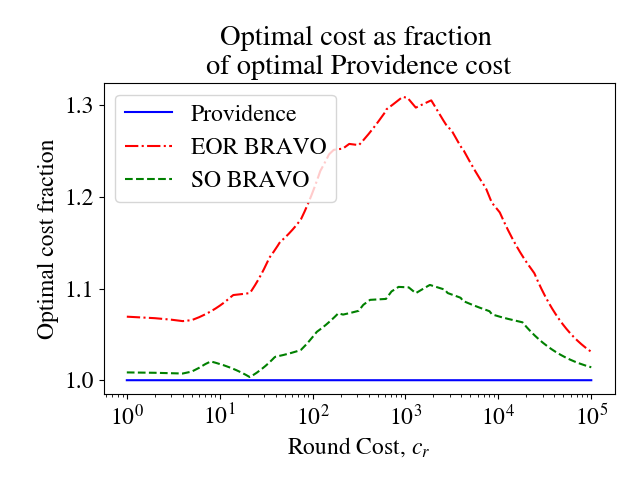
\includegraphics[width=.5\textwidth]{optimal_workloads.png}
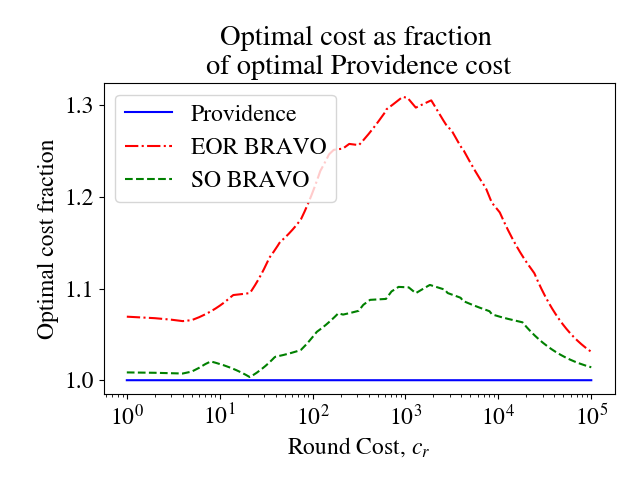
\includegraphics[width=.5\textwidth]{optimal_workloads.png}
\caption{For varying round workload $w_r$, the optimal average workload achievable by each audit, as a fraction of the \Providence values.}
\label{fig:optimal_workloads}
\end{figure}

Figure~\ref{fig:optimal_ps} shows the corresponding round schedule parameters $p$ that achieve these minimal workloads. As expected, an overhead for each round means that larger round sizes are needed to achieve an optimal audit, and so for all three audits $p$ increases as a function of $w_r$. Notice that \Providence is generally above and to the left of SO \BRAVO, and SO \BRAVO is generally above and to the left of EoR \BRAVO. This relationship reflects the fact that for the same round workload, \Providence can get away with a larger stopping probability because it requires fewer ballots.
\begin{figure}[h!]
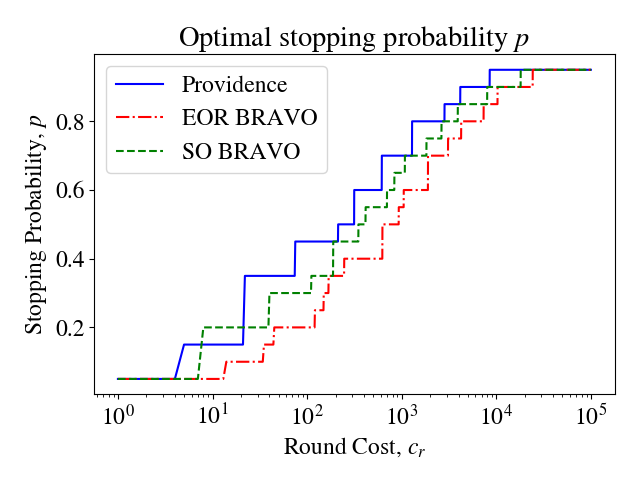
\includegraphics[width=.5\textwidth]{optimal_ps.png}
\caption{The optimal (workload-minimizing) stopping probability $p$ for varying workload model parameters $w_r$. (Note that the steps in this function are a consequence of our subsampling the workload function. That is, the workload-minimizing value of $p$ for each $w_r$ is only allowed to take on values at increments of $0.05$.)}
\label{fig:optimal_ps}
\end{figure}

\subsubsection{Precinct overhead.} For a more complete model, we can also introduce container-level workload. If a round requires multiple ballots from a single container, the container need only be unsealed once. Based on a Rhode Island pilot RLA report\cite{RI-report}, this may mean that a ballot from a new container requires roughly twice the time as a ballot from an already-opened container. Typically available election results give per-precinct granularity of vote tallies, rather than individual container information. In Virginia, however, most precincts have a single ballot scanner whose one box has sufficient capacity for all the ballots cast in that precinct anyways, and so we model the per-container workload as a per-precinct workload, $w_p$. In this model, the workload estimate incurs an additional workload of $w_p$ every time a precinct is sampled from for the first time in a round. That is, let $E_{pi}$ be the expected number of distinct precincts sampled from in round $i$, and let $E_p=\sum_i E_{pi}$. Then the new model is
\begin{equation}
W(E_b, E_r, E_p) = E_b w_b + E_r w_r + E_p w_p + C
\label{eq:round_and_precinct_workload}
\end{equation}

We can again explore the minimum achievable workloads under this model, as shown in Figure~\ref{fig:optimal_workload_precinct_workload_ratio}.

\begin{figure}
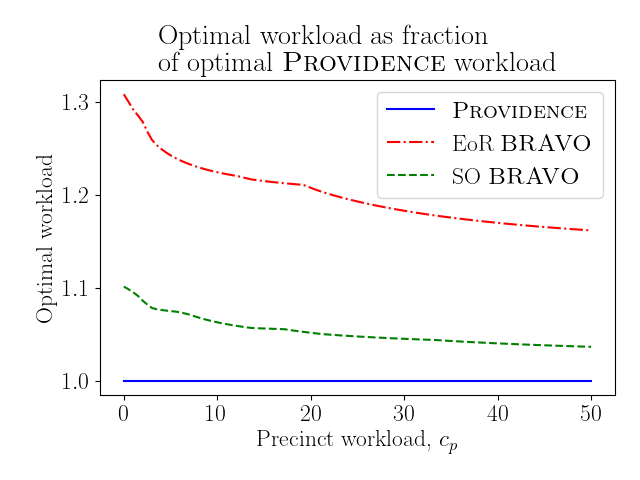
\includegraphics[width=.5\textwidth]{optimal_workload_precinct_workload_ratio.png}
\caption{Optimal average workload using the workload Equation~\ref{eq:round_and_precinct_workload} for varying $w_p$, given as a fraction of the value for \Providence. Similar to Figure~\ref{fig:optimal_workloads}, we show a generous range of values for the workload variable, $c_p$ in this case. If the time for a single ballot is $75$ seconds, then $c_p=50$ corresponds to over an hour of extra time to sample a ballot from a new container.}
\label{fig:optimal_workload_precinct_workload_ratio}
\end{figure}


\subsection{Real time}
Given tight certification deadlines,
%\footnote{Virginia recently passed legislation requiring pre-certification RLAs.}, 
the total real time to conduct the RLA is also an important factor to consider when planning audits.
Because each county can sample ballots for the same round concurrently, the total real time for a round depends only on the slowest county. 
In Virginia, Fairfax County typically has the most votes cast by a significant difference; in the contest we consider, Fairfax County had ~551 thousand votes cast, more than double the ~203 thousand of second-highest Virginia Beach City.
Consequently, we model the expected total real time $T$ of an audit using just the largest county, and we define analagous variables for the expected values in just the largest county.
Note that some other county may be slower, having fewer votes but also less auditing resources; but still, a slowest county exists. In this example, we take it to be Fairfax, the largest.
For the slowest county, let the expected total ballots sampled be $\bar E_b$, the expected number of rounds $\bar E_r$, and the expected number of distinct precinct samples summed over all rounds be $\bar E_p$.
Similarly, we use real time per-ballot, per-round, and per-precinct workload variables, $t_b$, $t_r$, and $t_p$. So the real time of the audit is estimated by
\begin{equation}
T(\bar E_b, \bar E_r, \bar E_p ) = \bar E_b t_b + \bar E_r t_r + \bar E_p t_p + C
\label{eq:real_time}
\end{equation}

As before, we can use our simulations to estimate $\bar E_b$, $\bar E_r$, and $\bar E_p$ using the corresponding averages over the trials. 
Available data to estimate values for $t_b$, $t_r$, and $t_p$ is limited, and so we take as an example the values $t_b=75$ seconds, $t_r=3$ hours, and $t_p=75$ seconds\footnote{The value $t_b=75$ seconds corresponds to a serial retrieval and interpretation of the ballots based on the \cite{RI-report} timing, $t_p=75$ seconds corresponds to the approximate doubling in time for new-box ballots as reported in \cite{RI-report} in the ballot-level comparison timing data, and $t_r=3$ hours is just a guess at an approximate order of magnitude for this variable.}. In practice, election officials could use our software and their own estimates of these values to explore choices for round schedules. Figure~\ref{fig:real_time} shows how the estimated real time for these values differs as a function of $p$. It should be noted that real values of $t_b$, $t_r$, and $t_p$ will vary greatly based on the number of parallel teams retrieving and checking ballots, the distribution of ballots and containers both in number and physical space, and other factors. We provide Figure~\ref{fig:real_time} only as an example of the general shape and behavior of this function. Use of this optimal scheduling tool would depend on parameter estimates tailored to each case.

\begin{figure}
%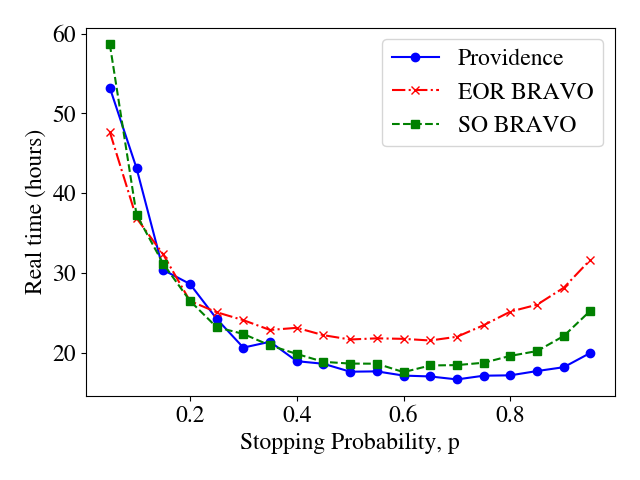
\includegraphics[width=.5\textwidth]{real_time.png}
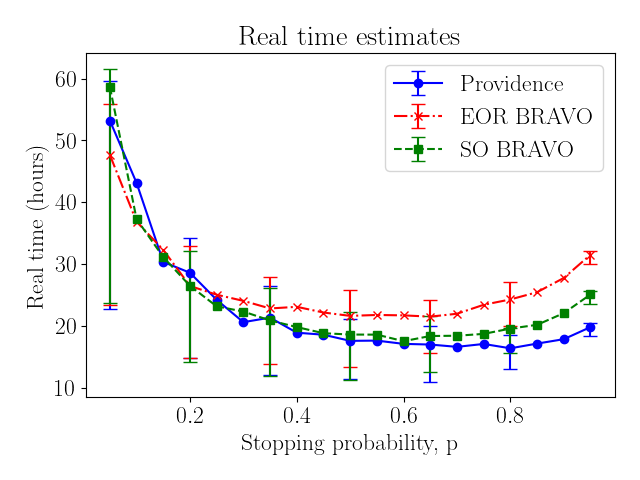
\includegraphics[width=.5\textwidth]{real_time_errorbars.png}
\caption{The real time as estimated by Equation~\ref{eq:real_time} for varying $p$ with expected values as estimated by our simulations. Error bars show the $0.25$ and $0.75$ quantiles. Unlike Figures \ref{fig:avg_bals} and \ref{fig:with_round_workload}, the quantiles still differ for large $p$ because the first round size is no longer a constant; the number of ballots drawn in the first round in Fairfax County is variable.}
\label{fig:real_time}
\end{figure}


\section{Misleading samples}
\label{sec:misleading}

Unfortunately, efficiency alone is not sufficient for planning audits. In the US today, election officials have a legitimate need to include personal safety as a consideration.
In a random sample, a true loser may receive more votes than the true winner. This happens more often when the sample sizes are small, like for a hypothetical first round size of $11$ in the pilot audit, as seen in Figure~\ref{fig:pilot_sequence}.
In the abstract, a misleading sample in an early round is dealt with by drawing more ballots (moving on to another round), but in practice it serves to create expectations or suspicions that then need to be managed by election officials. Hence there is reason to structure round sizes so that they are unlikely to misrepresent the true outcome.

%, angry supporters of the losing candidate may be suspicious of election officials moving onto a next round, or, if the audit is declared correct after the second round, feel sufficiently disappointed to pose a threat. 
%but in practice the implications of this approach may be dangerous.

%Imagine that Alice beats Bob in an election contest both truly and in the reported results, but Bob's supporters are insistent he really won. When election officials carry out the RLA, they choose a small first round size in the hopes of achieving an efficient audit by getting to stop sooner (and drawing fewer ballots on average). 
% After the first round, by chance, there are more votes for Bob than for Alice in the sample. Bob's supporters celebrate their victory that the audit has in fact revealed that Bob really won, but the election officials have to explain that they are moving on to a second round. 

%After the second round, there are more votes in the sample for Alice and sufficiently many that the risk limit is met and the audit now ends confirming the announced result that Alice won. This is an undesirable situation, as it can appear to Bob's supporters that election officials are simply drawing ballots till a chosen outcome is obtained. 

We introduce the notion of a \emph{misleading sample}, any cumulative sample which, assuming the announced outcome is correct, contains more ballots for a loser than for the winner.
We can again use our simulations to gain insight into the frequency of \emph{misleading samples}.
For each stopping probability $p$, Figure~\ref{fig:misleading} gives the proportion of simulated audits that had a \emph{misleading sample} at any point. 
Notably, this proportion is as high as 1 in 5 for the smaller stopping probability round schedules.
Accordingly, we introduce a new parameter to our audit-planning tool, the maximum acceptable probability that the audit is misleading, the \emph{misleading limit}.

In Figure~\ref{fig:misleading}, horizontal lines are included to show \emph{misleading limits} of $0.1$, $0.01$, and $0.001$.
To achieve a probability of a misleading sample of at most $0.1$, a round schedule with at least roughly $p=.3$ is needed.
To achieve a probability of misleading of roughly $0.01$, a round schedule with $p=0.8$ is needed, and to achieve a probability of misleading of roughly $0.001$, a round schedule with $p=0.95$ is needed.
It is not unreasonable to think that election officials might choose a \emph{misleading limit} of $0.01$, or smaller, given the state of public perception of election security in the US and the associated threats of violence.
Consequently, the desired \emph{misleading limit} may be a deciding constraint in the choice of round schedule. 

\begin{figure}
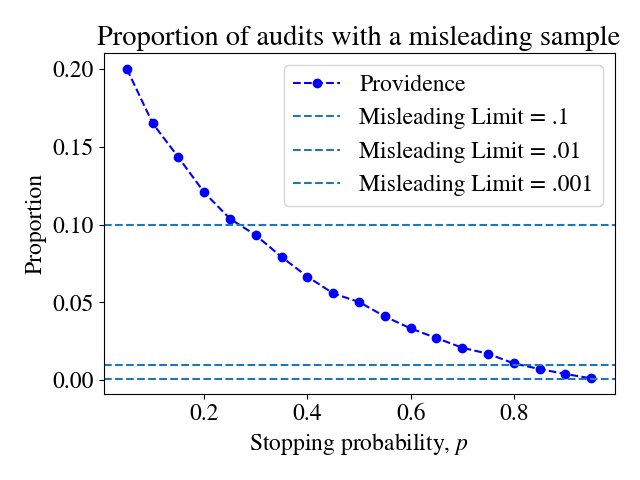
\includegraphics[width=.5\textwidth]{misleading_limits.png}
%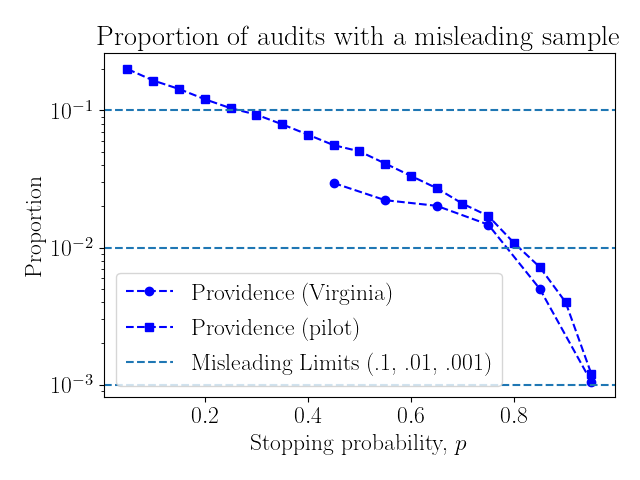
\includegraphics[width=.5\textwidth]{combined_misleading.png}
\caption{The proportion of simulated \Providence audits for the Virginia and pilot contest parameters that had a \emph{misleading sample} in any round.}
\label{fig:misleading}
\end{figure}

%We observe a similar behavior in our simulations of audits on the contest from the pilot audit. Figure~\ref{fig:misleading} also shows the proportion of the pilot simulations which contained a \emph{misleading sample} in any round. Despite the large difference in margin ($\sim 0.05$ in Virginia and $\sim 0.25$ in the pilot) we still observe that a \emph{misleading limit} of $0.01$ is first achieved at roughly $p=0.8$ and $0.001$ at $p=0.95$.

%\begin{figure}
%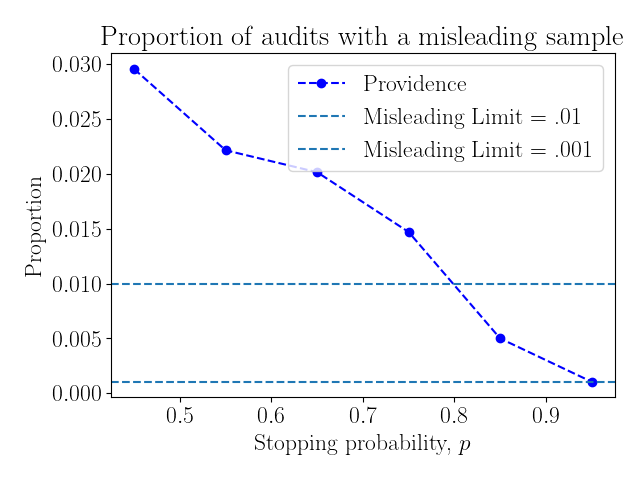
\includegraphics[width=.5\textwidth]{pilot_misleading_prop.png}
%\caption{The proportion of simulated \Providence audits for the pilot audit parameters that had a \emph{misleading sample} in any round.}
%\label{fig:pilot_misleading}
%\end{figure}

If election officials wish to enforce a \emph{misleading limit} for all the rounds, our simulation analysis could help. On the other hand, for a given round, it is straightforward to compute analytically the probability that a loser has more votes than the winner in the sample. Table~\ref{tab:misleading} shows for various margins the minimum first round size $n$ that guarantees a probability of a \emph{misleading sample} at most $M\in\{0.1,0.01,0.001\}$. For all values of $M$ and all margins, \Providence achieves a higher probability of stopping than either EoR \BRAVO or SO \BRAVO. 
    As seen in the Table~\ref{tab:misleading}, to enforce $M=0.01$ requires minimum round sizes with at least roughly a $0.8$ probability of stopping in the first round. Even if the most efficient audit schedule (by either workload or real time measures) would use a lower stopping probability $p$ to choose the first round size, the election officials may opt to use this constraint on the probability of a \emph{misleading sample} as the deciding factor in planning their audits.